\documentclass[10pt,hyperref={colorlinks,citecolor=blue,urlcolor=peking_blue,linkcolor=}]{beamer}
\usepackage{Bydevmar}
\usefonttheme{serif}
\usepackage{lipsum}
%\usepackage[scheme = plain]{ctex}
\usepackage{hyperref}
\usepackage{charter} % Nicer fonts
% other packages
\usepackage{latexsym,amsmath,xcolor,multicol,booktabs,calligra}
\usepackage{amssymb}
\usepackage{graphicx}
\usepackage{bm}
\usepackage{natbib}
\usepackage{wrapfig}
\usepackage{amsfonts} 
\usepackage{ragged2e}
\usepackage{parskip}

\apptocmd{\frame}{}{\justifying}{} % Allow optional arguments after frame.

\newcommand{\theHalgorithm}{\arabic{algorithm}}
\theoremstyle{plain}
\newtheorem{axiom}{Axiom}
\newtheorem{claim}[axiom]{Claim}
\newtheorem{assumption}{Assumption}
\newtheorem{remark}{Remark}
\newtheorem{proposition}{Proposition}
\setbeamertemplate{theorems}[numbered] 


% change for your title page information
\author[FPO]{Faculté Polydisciplinaire - Ouarzazate}
\title{LA CONNÉCTIVITÉ LA THÉORIE DE MENGER EN THÉORIE DES GPRAPHES}
\subtitle{Module : Théorie des graphes}
\institute{Master Mathématiques Appliquées pour la Science des Données}
\date{
2024/05/04}

\newif\ifplacelogo % create a new conditional
\placelogotrue % set it to true
\logo{
\ifplacelogo
\includegraphics[width=2cm]{../Figures/PKU-China-logo.png}
\fi
}
% official colors match with the PKU red
\def\cmd#1{\texttt{\color{red}\footnotesize $\backslash$#1}}
\def\env#1{\texttt{\color{blue}\footnotesize #1}}
\definecolor{deepblue}{rgb}{0,0,0.5}
\definecolor{deepred}{rgb}{0.6,0,0}
\definecolor{deepgreen}{rgb}{0,0.5,0}
\definecolor{halfgray}{gray}{0.55}


\usepackage{tcolorbox}

% Définition de la couleur orange
\definecolor{orange}{RGB}{255,140,0}
\begin{document}
{
\setbeamertemplate{logo}{}
\begin{frame}
    \titlepage
    \begin{figure}[htpb]
        \begin{center}
            
\includegraphics[width=0.7\linewidth]{Figures/fpo_logo.png}
        \end{center}
    \end{figure}
\end{frame}
}

\placelogofalse

%%%%%%%%%%%
% Concepts Introductifs
%%%%%%%%%%%
\section{Concepts Introductifs}



\begin{frame}{Détection de fraude}
    \begin{center}
        \colorbox{white}{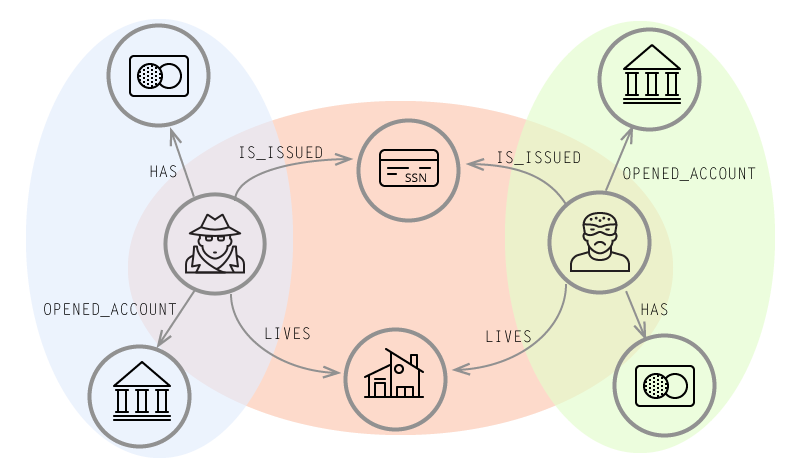
\includegraphics[width=0.8\textwidth]{img/usecase-fraud.png}}
\end{center}
\end{frame}


\begin{frame}
\frametitle{Connectivité dans les Graphes : Variétés, Implications et Exemples}
    \begin{tcolorbox}[colback=orange!10,colframe=orange!100!black,
        title=La connectivité dans les graphes]
        La connectivité dans les graphes a des implications variées dans de nombreux domaines, tels que les réseaux informatiques, la planification urbaine et la biologie. Elle est définie comme suit :
        \begin{itemize}
            \item \textbf{Connectivité de sommets ($\kappa$)}: Le nombre minimum de sommets dont la suppression entraîne un graphe non connexe ou réduit le graphe à un seul sommet.
            \item \textbf{Connectivité d'arêtes ($\lambda$)}: Le nombre minimum d'arêtes dont la suppression rend le graphe non connexe.
        \end{itemize}
        Ces deux mesures sont liées par l'inégalité suivante :
        $$ \kappa(G) \leq \lambda(G) \leq \delta(G) $$
        où $\delta(G)$ est le degré minimum d'un sommet dans le graphe $G$.
    \end{tcolorbox}
\end{frame}

\begin{frame}{	CLI Neo4j Command Line Interface}
  \begin{block}{cli neo4 j}
    	CLI Neo4j (Command Line Interface) :
\begin{itemize}
   
	\item Pour exécuter une requête Cypher, vous pouvez utiliser la commande cypher suivie de votre requête. Par exemple : cypher "MATCH (n) RETURN n"
\item	Pour gérer les utilisateurs et les autorisations, vous pouvez utiliser les commandes user et role.
\item	Pour importer des données, utilisez la commande import.
\item	Pour surveiller et configurer votre instance Neo4j, vous pouvez utiliser des commandes telles que info, metrics, set, etc.
\end{itemize}
  \end{block}
  
\end{frame}
\begin{frame}
\frametitle{Exploration de la Connectivité des Graphes : Théorème de Menger}
\begin{tcolorbox}[colback=orange!10,colframe=orange!100!black,
    title=\textbf{Théorème de Menger}]
    Le théorème de Menger est un résultat fondamental en théorie des graphes qui établit une relation entre la connectivité locale et globale d'un graphe. Il stipule que pour deux sommets non adjacents \( u \) et \( v \) dans un graphe, le nombre minimum de sommets à supprimer pour séparer \( u \) et \( v \) est égal au nombre maximum de chemins indépendants de \( u \) à \( v \).
    
    Formellement, la formule mathématique est donnée par :
    $$ \kappa(u,v) = \max \{ \text{nombre de chemins indépendants de } u \text{ à } v \} $$
    où \( \kappa(u,v) \) représente la connectivité entre les sommets \( u \) et \( v \).
\end{tcolorbox}
\end{frame}

\begin{frame}
\frametitle{Application Pratique : Théorème de Menger}
\begin{tcolorbox}[colback=orange!10,colframe=orange!100!black,
    title=\textbf{Exemple du Théorème de Menger}]
    Considérons un graphe où les sommets \( A \) et \( B \) ne sont pas adjacents. Selon le théorème de Menger, pour déterminer le nombre minimum de sommets à supprimer pour séparer \( A \) de \( B \), nous devons trouver le nombre maximum de chemins indépendants de \( A \) à \( B \).

    Supposons qu'il y ait trois chemins indépendants entre \( A \) et \( B \). Alors, selon le théorème de Menger, nous devons supprimer au moins trois sommets pour séparer \( A \) de \( B \).

    La formule mathématique s'applique comme suit :
    $$ \kappa(A,B) = 3 $$
    Ce qui signifie que la connectivité \( \kappa \) entre \( A \) et \( B \) est de trois, et donc trois est le nombre minimum de sommets à supprimer pour les séparer.
\end{tcolorbox}
\end{frame}




\begin{frame}{ \textbf{Example  Importation à partir de fichiers CSV}}
\textit{}{\textbf{Fichier CSV :}}  
    \begin{center}
        \begin{tabular}{|l|l|l|}
            \hline
           name & ville& age \\
            \hline
            hassan & casa& 25 \\
           walid & fes  & 23 \\
           fatima & agadir & 65 \\
            \hline
        \end{tabular}
    \end{center}
    
 \begin{block}{cypher}
 LOAD CSV WITH HEADERS FROM 'file:///employees.csv' AS row
CREATE (:person { name: row.name, ville: row.ville, age: toInteger(row.age)})

  \end{block}
\end{frame}    
\begin{frame}{La loi Dodd-Frank et son impact sur la réglementation Q}
   La loi Dodd-Frank a abrogé le règlement Q, autorisant les banques à payer des intérêts sur les dépôts à vue pour la première fois depuis plus de 70 ans. Ce changement a été perçu comme une évolution positive par beaucoup, car il offre aux consommateurs davantage d’options pour épargner et gagner des intérêts. Cependant, certains craignaient que l'abrogation du règlement Q puisse également conduire à une prise de risque accrue de la part des banques, dans la mesure où elles seraient désormais en mesure d'offrir des taux de dépôt plus élevés pour attirer les clients. 
\end{frame}
\begin{frame}
\frametitle{Définitions Fondamentales des Graphes}

\begin{tcolorbox}[colback=orange!10,colframe=orange!100!black,
    title=Un Cycle]
    Un \textbf{Cycle} est un chemin qui commence et se termine au même sommet.
\end{tcolorbox}

\begin{figure}[H]
    \centering
    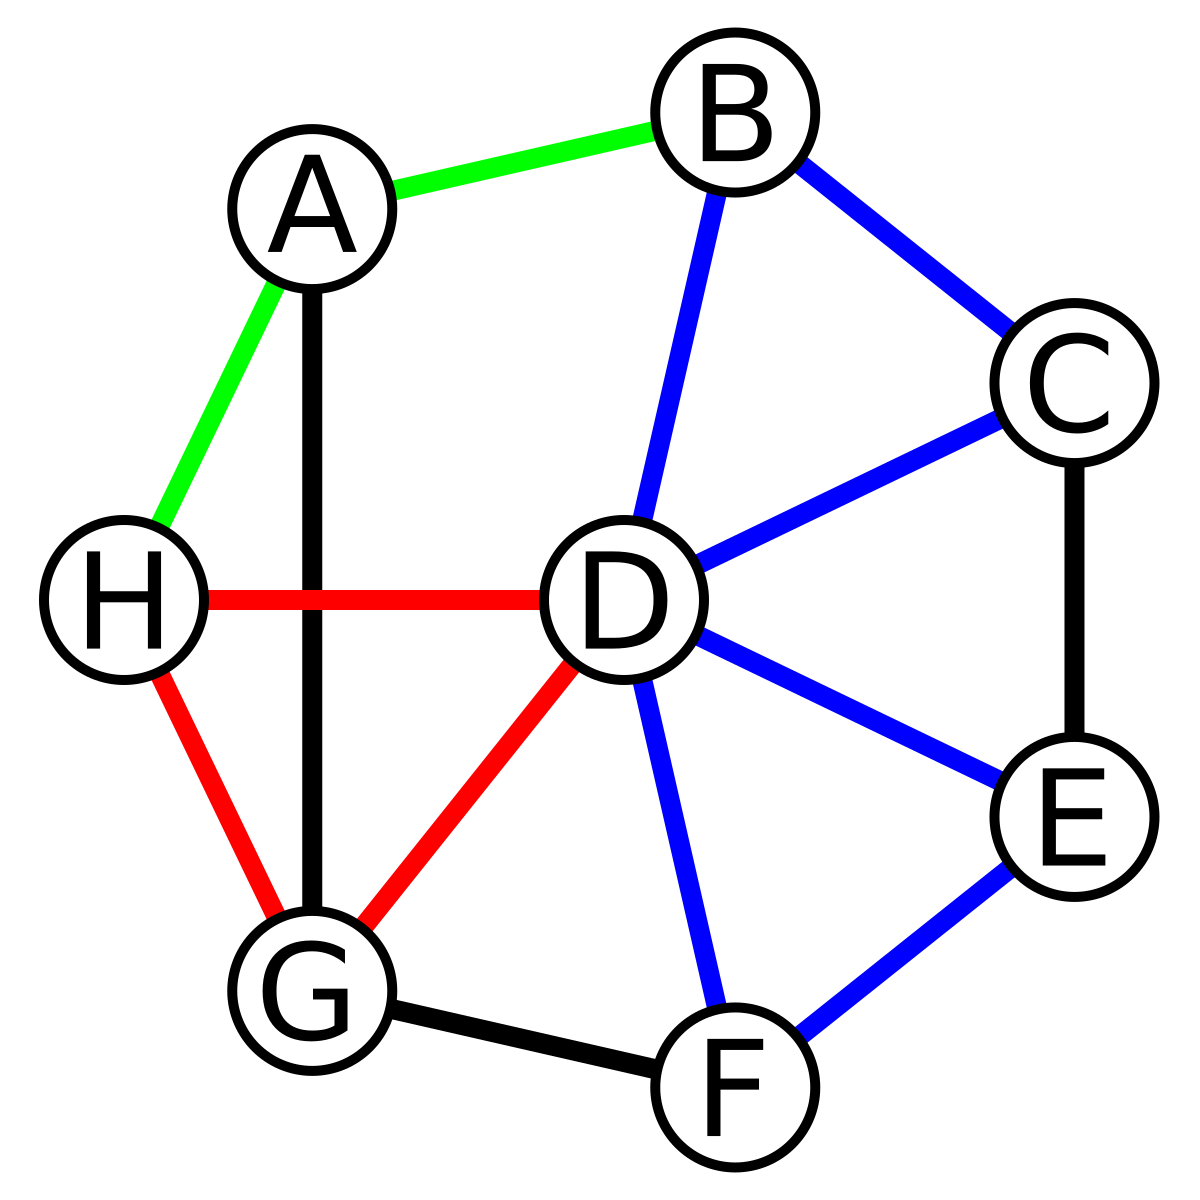
\includegraphics[width=0.5 \textwidth]{Figures/cycle.png}
    \caption{Un Cycle}
    \label{fig:Un Cycle}
\end{figure}

\end{frame}

\begin{frame}{les instruments financiers et la loi Dodd-Frank }


Avant Dodd-Frank, les instruments financiers manquaient de régulation, exposant à l'opacité et aux abus. Les dérivés étaient utilisés sans contrôle, alimentant l'instabilité. Dodd-Frank a transformé cela en imposant la transparence des dérivés, renforçant la surveillance avec des organismes comme le FSOC et protégeant les consommateurs. Les exigences plus strictes ont également renforcé la stabilité financière. Ainsi, Dodd-Frank a rendu les instruments financiers plus sûrs et mieux réglementés.
\end{frame}
\begin{frame}{Exécution de requêtes en direct}
  \begin{block}{Trouver tous les joueurs d'une équipe}
    \begin{itemize}
      \item MATCH (j:Joueur)-[:JOUE\_POUR]->(e:Equipe {nom: 'PSG'});
      \item RETURN j.nom, j.prenom, j.age;
    \end{itemize}
    Cette requête retourne les noms, prénoms et âges de tous les joueurs qui jouent pour le PSG.
  \end{block}
  \begin{block}{Trouver l'entraîneur d'une équipe}
    \begin{itemize}
      \item MATCH (e:Equipe {nom: 'FCB'})<-[:ENTRAINE]-(entraineur);
      \item RETURN entraineur.nom;
    \end{itemize}
    Cette requête retourne le nom de l'entraîneur du FC Barcelone.
  \end{block}
\end{frame}
%%%%%%%%%%%%%%%%%%%%%%%%%%%%%%%


%%%%%%%%%%%
% Theoreme De Menger
%%%%%%%%%%%
\section{Concepts Introductifs}



\begin{frame}{Détection de fraude}
    \begin{center}
        \colorbox{white}{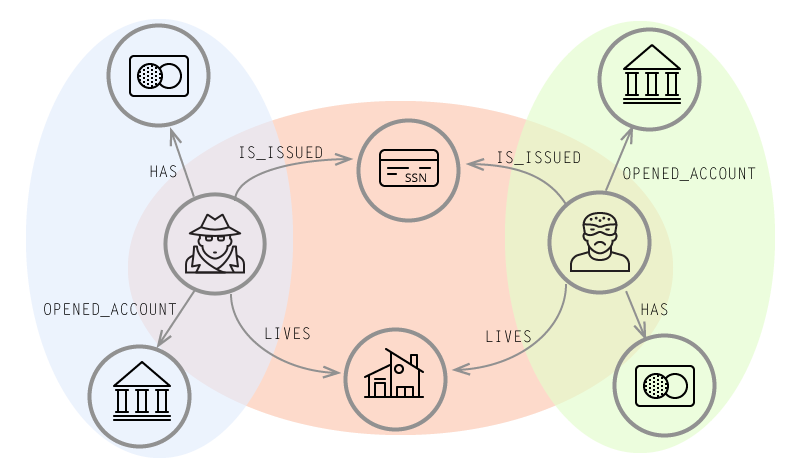
\includegraphics[width=0.8\textwidth]{img/usecase-fraud.png}}
\end{center}
\end{frame}


\begin{frame}
\frametitle{Connectivité dans les Graphes : Variétés, Implications et Exemples}
    \begin{tcolorbox}[colback=orange!10,colframe=orange!100!black,
        title=La connectivité dans les graphes]
        La connectivité dans les graphes a des implications variées dans de nombreux domaines, tels que les réseaux informatiques, la planification urbaine et la biologie. Elle est définie comme suit :
        \begin{itemize}
            \item \textbf{Connectivité de sommets ($\kappa$)}: Le nombre minimum de sommets dont la suppression entraîne un graphe non connexe ou réduit le graphe à un seul sommet.
            \item \textbf{Connectivité d'arêtes ($\lambda$)}: Le nombre minimum d'arêtes dont la suppression rend le graphe non connexe.
        \end{itemize}
        Ces deux mesures sont liées par l'inégalité suivante :
        $$ \kappa(G) \leq \lambda(G) \leq \delta(G) $$
        où $\delta(G)$ est le degré minimum d'un sommet dans le graphe $G$.
    \end{tcolorbox}
\end{frame}

\begin{frame}{	CLI Neo4j Command Line Interface}
  \begin{block}{cli neo4 j}
    	CLI Neo4j (Command Line Interface) :
\begin{itemize}
   
	\item Pour exécuter une requête Cypher, vous pouvez utiliser la commande cypher suivie de votre requête. Par exemple : cypher "MATCH (n) RETURN n"
\item	Pour gérer les utilisateurs et les autorisations, vous pouvez utiliser les commandes user et role.
\item	Pour importer des données, utilisez la commande import.
\item	Pour surveiller et configurer votre instance Neo4j, vous pouvez utiliser des commandes telles que info, metrics, set, etc.
\end{itemize}
  \end{block}
  
\end{frame}
\begin{frame}
\frametitle{Exploration de la Connectivité des Graphes : Théorème de Menger}
\begin{tcolorbox}[colback=orange!10,colframe=orange!100!black,
    title=\textbf{Théorème de Menger}]
    Le théorème de Menger est un résultat fondamental en théorie des graphes qui établit une relation entre la connectivité locale et globale d'un graphe. Il stipule que pour deux sommets non adjacents \( u \) et \( v \) dans un graphe, le nombre minimum de sommets à supprimer pour séparer \( u \) et \( v \) est égal au nombre maximum de chemins indépendants de \( u \) à \( v \).
    
    Formellement, la formule mathématique est donnée par :
    $$ \kappa(u,v) = \max \{ \text{nombre de chemins indépendants de } u \text{ à } v \} $$
    où \( \kappa(u,v) \) représente la connectivité entre les sommets \( u \) et \( v \).
\end{tcolorbox}
\end{frame}

\begin{frame}
\frametitle{Application Pratique : Théorème de Menger}
\begin{tcolorbox}[colback=orange!10,colframe=orange!100!black,
    title=\textbf{Exemple du Théorème de Menger}]
    Considérons un graphe où les sommets \( A \) et \( B \) ne sont pas adjacents. Selon le théorème de Menger, pour déterminer le nombre minimum de sommets à supprimer pour séparer \( A \) de \( B \), nous devons trouver le nombre maximum de chemins indépendants de \( A \) à \( B \).

    Supposons qu'il y ait trois chemins indépendants entre \( A \) et \( B \). Alors, selon le théorème de Menger, nous devons supprimer au moins trois sommets pour séparer \( A \) de \( B \).

    La formule mathématique s'applique comme suit :
    $$ \kappa(A,B) = 3 $$
    Ce qui signifie que la connectivité \( \kappa \) entre \( A \) et \( B \) est de trois, et donc trois est le nombre minimum de sommets à supprimer pour les séparer.
\end{tcolorbox}
\end{frame}




\begin{frame}{ \textbf{Example  Importation à partir de fichiers CSV}}
\textit{}{\textbf{Fichier CSV :}}  
    \begin{center}
        \begin{tabular}{|l|l|l|}
            \hline
           name & ville& age \\
            \hline
            hassan & casa& 25 \\
           walid & fes  & 23 \\
           fatima & agadir & 65 \\
            \hline
        \end{tabular}
    \end{center}
    
 \begin{block}{cypher}
 LOAD CSV WITH HEADERS FROM 'file:///employees.csv' AS row
CREATE (:person { name: row.name, ville: row.ville, age: toInteger(row.age)})

  \end{block}
\end{frame}    
\begin{frame}{La loi Dodd-Frank et son impact sur la réglementation Q}
   La loi Dodd-Frank a abrogé le règlement Q, autorisant les banques à payer des intérêts sur les dépôts à vue pour la première fois depuis plus de 70 ans. Ce changement a été perçu comme une évolution positive par beaucoup, car il offre aux consommateurs davantage d’options pour épargner et gagner des intérêts. Cependant, certains craignaient que l'abrogation du règlement Q puisse également conduire à une prise de risque accrue de la part des banques, dans la mesure où elles seraient désormais en mesure d'offrir des taux de dépôt plus élevés pour attirer les clients. 
\end{frame}
\begin{frame}
\frametitle{Définitions Fondamentales des Graphes}

\begin{tcolorbox}[colback=orange!10,colframe=orange!100!black,
    title=Un Cycle]
    Un \textbf{Cycle} est un chemin qui commence et se termine au même sommet.
\end{tcolorbox}

\begin{figure}[H]
    \centering
    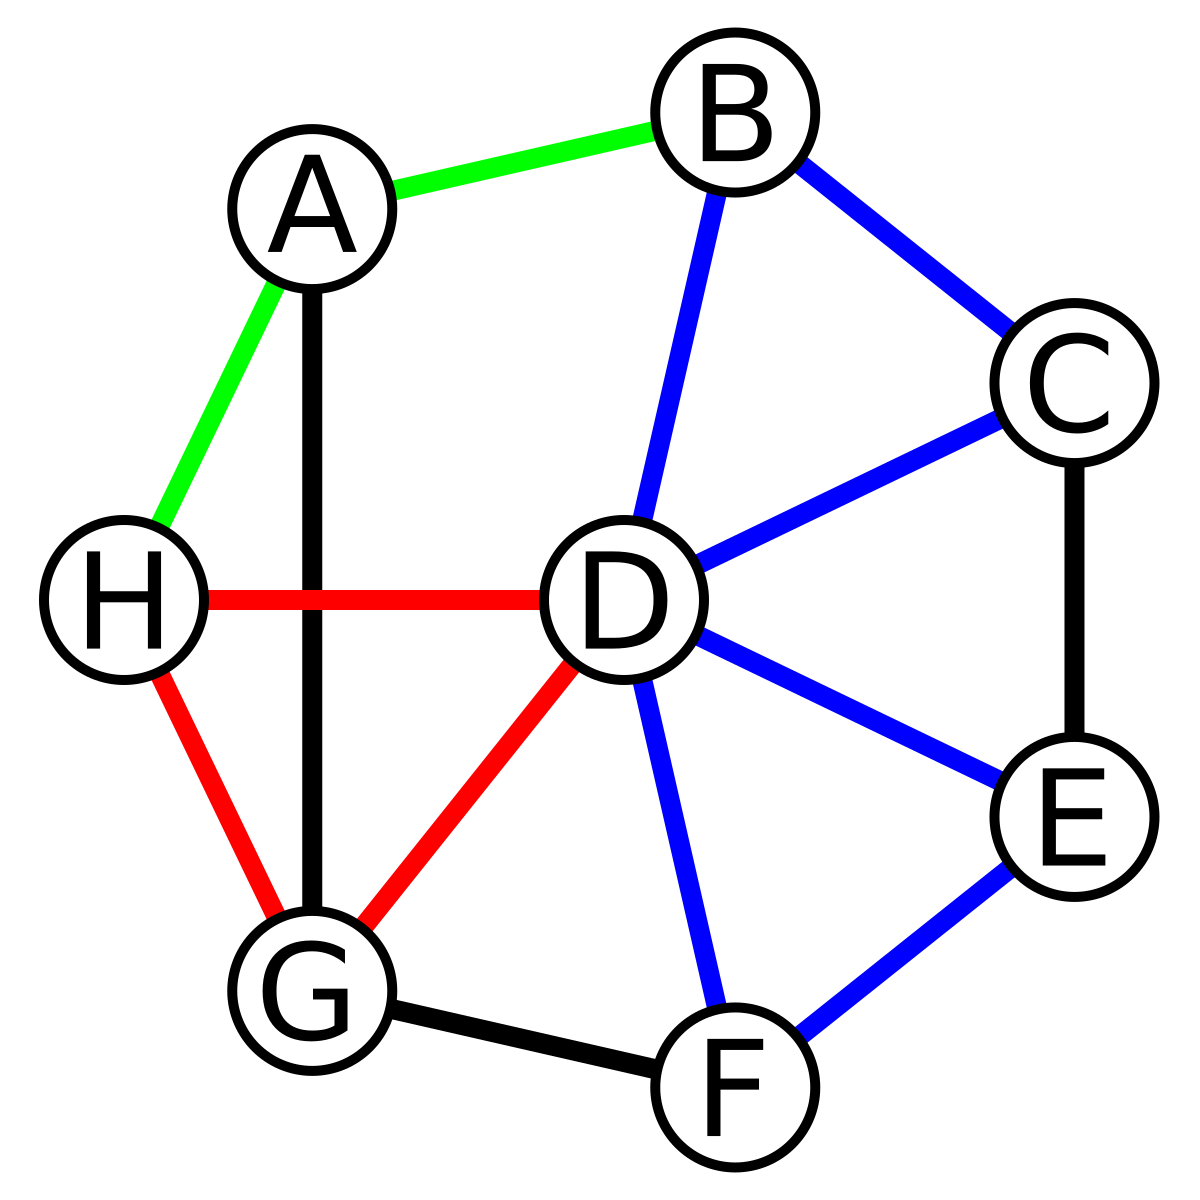
\includegraphics[width=0.5 \textwidth]{Figures/cycle.png}
    \caption{Un Cycle}
    \label{fig:Un Cycle}
\end{figure}

\end{frame}

\begin{frame}{les instruments financiers et la loi Dodd-Frank }


Avant Dodd-Frank, les instruments financiers manquaient de régulation, exposant à l'opacité et aux abus. Les dérivés étaient utilisés sans contrôle, alimentant l'instabilité. Dodd-Frank a transformé cela en imposant la transparence des dérivés, renforçant la surveillance avec des organismes comme le FSOC et protégeant les consommateurs. Les exigences plus strictes ont également renforcé la stabilité financière. Ainsi, Dodd-Frank a rendu les instruments financiers plus sûrs et mieux réglementés.
\end{frame}
\begin{frame}{Exécution de requêtes en direct}
  \begin{block}{Trouver tous les joueurs d'une équipe}
    \begin{itemize}
      \item MATCH (j:Joueur)-[:JOUE\_POUR]->(e:Equipe {nom: 'PSG'});
      \item RETURN j.nom, j.prenom, j.age;
    \end{itemize}
    Cette requête retourne les noms, prénoms et âges de tous les joueurs qui jouent pour le PSG.
  \end{block}
  \begin{block}{Trouver l'entraîneur d'une équipe}
    \begin{itemize}
      \item MATCH (e:Equipe {nom: 'FCB'})<-[:ENTRAINE]-(entraineur);
      \item RETURN entraineur.nom;
    \end{itemize}
    Cette requête retourne le nom de l'entraîneur du FC Barcelone.
  \end{block}
\end{frame}
%%%%%%%%%%%%%%%%%%%%%%%%%%%%%%%


%%%%%%%%%%%
% Distance et Connexite
%%%%%%%%%%%
\section{Concepts Introductifs}



\begin{frame}{Détection de fraude}
    \begin{center}
        \colorbox{white}{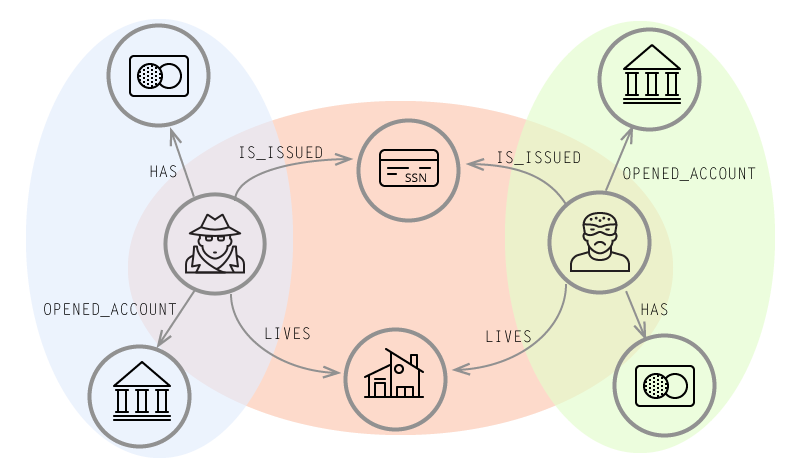
\includegraphics[width=0.8\textwidth]{img/usecase-fraud.png}}
\end{center}
\end{frame}


\begin{frame}
\frametitle{Connectivité dans les Graphes : Variétés, Implications et Exemples}
    \begin{tcolorbox}[colback=orange!10,colframe=orange!100!black,
        title=La connectivité dans les graphes]
        La connectivité dans les graphes a des implications variées dans de nombreux domaines, tels que les réseaux informatiques, la planification urbaine et la biologie. Elle est définie comme suit :
        \begin{itemize}
            \item \textbf{Connectivité de sommets ($\kappa$)}: Le nombre minimum de sommets dont la suppression entraîne un graphe non connexe ou réduit le graphe à un seul sommet.
            \item \textbf{Connectivité d'arêtes ($\lambda$)}: Le nombre minimum d'arêtes dont la suppression rend le graphe non connexe.
        \end{itemize}
        Ces deux mesures sont liées par l'inégalité suivante :
        $$ \kappa(G) \leq \lambda(G) \leq \delta(G) $$
        où $\delta(G)$ est le degré minimum d'un sommet dans le graphe $G$.
    \end{tcolorbox}
\end{frame}

\begin{frame}{	CLI Neo4j Command Line Interface}
  \begin{block}{cli neo4 j}
    	CLI Neo4j (Command Line Interface) :
\begin{itemize}
   
	\item Pour exécuter une requête Cypher, vous pouvez utiliser la commande cypher suivie de votre requête. Par exemple : cypher "MATCH (n) RETURN n"
\item	Pour gérer les utilisateurs et les autorisations, vous pouvez utiliser les commandes user et role.
\item	Pour importer des données, utilisez la commande import.
\item	Pour surveiller et configurer votre instance Neo4j, vous pouvez utiliser des commandes telles que info, metrics, set, etc.
\end{itemize}
  \end{block}
  
\end{frame}
\begin{frame}
\frametitle{Exploration de la Connectivité des Graphes : Théorème de Menger}
\begin{tcolorbox}[colback=orange!10,colframe=orange!100!black,
    title=\textbf{Théorème de Menger}]
    Le théorème de Menger est un résultat fondamental en théorie des graphes qui établit une relation entre la connectivité locale et globale d'un graphe. Il stipule que pour deux sommets non adjacents \( u \) et \( v \) dans un graphe, le nombre minimum de sommets à supprimer pour séparer \( u \) et \( v \) est égal au nombre maximum de chemins indépendants de \( u \) à \( v \).
    
    Formellement, la formule mathématique est donnée par :
    $$ \kappa(u,v) = \max \{ \text{nombre de chemins indépendants de } u \text{ à } v \} $$
    où \( \kappa(u,v) \) représente la connectivité entre les sommets \( u \) et \( v \).
\end{tcolorbox}
\end{frame}

\begin{frame}
\frametitle{Application Pratique : Théorème de Menger}
\begin{tcolorbox}[colback=orange!10,colframe=orange!100!black,
    title=\textbf{Exemple du Théorème de Menger}]
    Considérons un graphe où les sommets \( A \) et \( B \) ne sont pas adjacents. Selon le théorème de Menger, pour déterminer le nombre minimum de sommets à supprimer pour séparer \( A \) de \( B \), nous devons trouver le nombre maximum de chemins indépendants de \( A \) à \( B \).

    Supposons qu'il y ait trois chemins indépendants entre \( A \) et \( B \). Alors, selon le théorème de Menger, nous devons supprimer au moins trois sommets pour séparer \( A \) de \( B \).

    La formule mathématique s'applique comme suit :
    $$ \kappa(A,B) = 3 $$
    Ce qui signifie que la connectivité \( \kappa \) entre \( A \) et \( B \) est de trois, et donc trois est le nombre minimum de sommets à supprimer pour les séparer.
\end{tcolorbox}
\end{frame}




\begin{frame}{ \textbf{Example  Importation à partir de fichiers CSV}}
\textit{}{\textbf{Fichier CSV :}}  
    \begin{center}
        \begin{tabular}{|l|l|l|}
            \hline
           name & ville& age \\
            \hline
            hassan & casa& 25 \\
           walid & fes  & 23 \\
           fatima & agadir & 65 \\
            \hline
        \end{tabular}
    \end{center}
    
 \begin{block}{cypher}
 LOAD CSV WITH HEADERS FROM 'file:///employees.csv' AS row
CREATE (:person { name: row.name, ville: row.ville, age: toInteger(row.age)})

  \end{block}
\end{frame}    
\begin{frame}{La loi Dodd-Frank et son impact sur la réglementation Q}
   La loi Dodd-Frank a abrogé le règlement Q, autorisant les banques à payer des intérêts sur les dépôts à vue pour la première fois depuis plus de 70 ans. Ce changement a été perçu comme une évolution positive par beaucoup, car il offre aux consommateurs davantage d’options pour épargner et gagner des intérêts. Cependant, certains craignaient que l'abrogation du règlement Q puisse également conduire à une prise de risque accrue de la part des banques, dans la mesure où elles seraient désormais en mesure d'offrir des taux de dépôt plus élevés pour attirer les clients. 
\end{frame}
\begin{frame}
\frametitle{Définitions Fondamentales des Graphes}

\begin{tcolorbox}[colback=orange!10,colframe=orange!100!black,
    title=Un Cycle]
    Un \textbf{Cycle} est un chemin qui commence et se termine au même sommet.
\end{tcolorbox}

\begin{figure}[H]
    \centering
    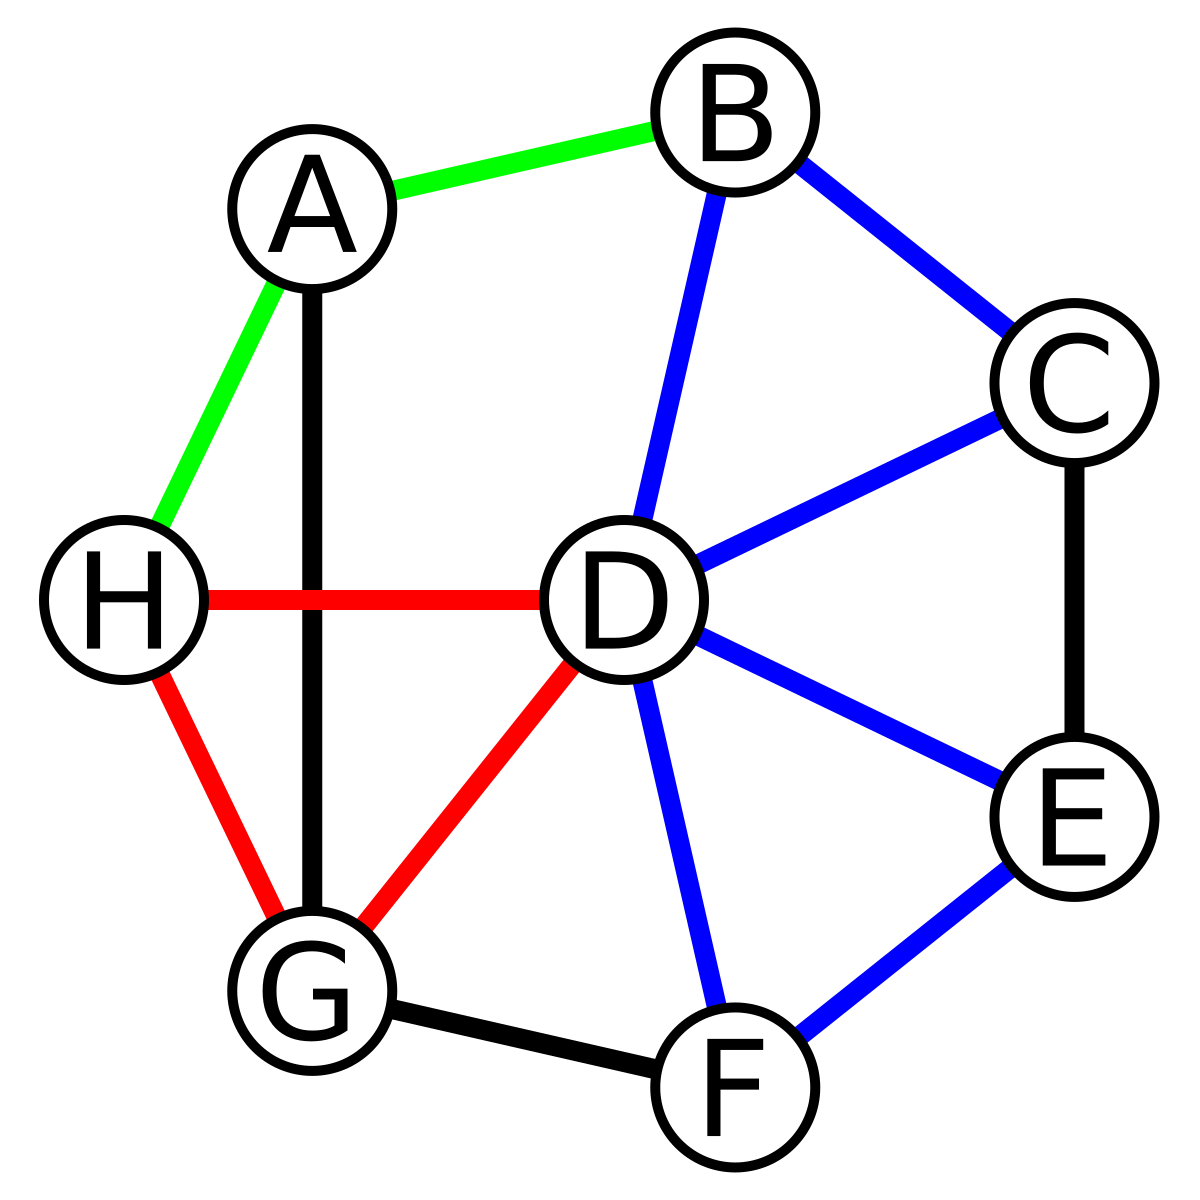
\includegraphics[width=0.5 \textwidth]{Figures/cycle.png}
    \caption{Un Cycle}
    \label{fig:Un Cycle}
\end{figure}

\end{frame}

\begin{frame}{les instruments financiers et la loi Dodd-Frank }


Avant Dodd-Frank, les instruments financiers manquaient de régulation, exposant à l'opacité et aux abus. Les dérivés étaient utilisés sans contrôle, alimentant l'instabilité. Dodd-Frank a transformé cela en imposant la transparence des dérivés, renforçant la surveillance avec des organismes comme le FSOC et protégeant les consommateurs. Les exigences plus strictes ont également renforcé la stabilité financière. Ainsi, Dodd-Frank a rendu les instruments financiers plus sûrs et mieux réglementés.
\end{frame}
\begin{frame}{Exécution de requêtes en direct}
  \begin{block}{Trouver tous les joueurs d'une équipe}
    \begin{itemize}
      \item MATCH (j:Joueur)-[:JOUE\_POUR]->(e:Equipe {nom: 'PSG'});
      \item RETURN j.nom, j.prenom, j.age;
    \end{itemize}
    Cette requête retourne les noms, prénoms et âges de tous les joueurs qui jouent pour le PSG.
  \end{block}
  \begin{block}{Trouver l'entraîneur d'une équipe}
    \begin{itemize}
      \item MATCH (e:Equipe {nom: 'FCB'})<-[:ENTRAINE]-(entraineur);
      \item RETURN entraineur.nom;
    \end{itemize}
    Cette requête retourne le nom de l'entraîneur du FC Barcelone.
  \end{block}
\end{frame}
%%%%%%%%%%%%%%%%%%%%%%%%%%%%%%%


%%%%%%%%%%%
% Distance et Connexite
%%%%%%%%%%%


\section{Conclusion}
\begin{frame}
\frametitle{Conclusion}
\begin{itemize}
    \item Le \textbf{théorème de Menger} est un concept central en théorie des graphes, essentiel pour comprendre la connectivité.
    \item Ses applications sont vastes, touchant des domaines tels que les réseaux informatiques, l'urbanisme et la biologie.
    \item La capacité à identifier les chemins indépendants et les points de vulnérabilité dans les réseaux peut conduire à des améliorations significatives dans la conception et la résilience des systèmes.
    \item Les concepts de connectivité et de distance dans les graphes continueront d'être des sujets de recherche pertinents pour résoudre des problèmes complexes dans diverses disciplines.
\end{itemize}
\textbf{Perspectives :} La poursuite de l'étude des graphes et de leurs propriétés est cruciale pour le développement de technologies et d'infrastructures plus robustes et efficaces à l'avenir.
\end{frame}

%%%%%%%%%%%%%%%%%%%%%%%%%%%%%%%
\end{document}